\begin{remark}
The classificator is linear ($G_1(x)=G_2(x)$ is a line) if the covariance matrices of both Gauss distributions are identical. This fact can be used to simplify the calculation, however, this usually is not an issue. On the other hand, if we assume the classifier is supposed to be linear, it can be used to calculate the covariance matrix from all the data at only (and not per category as it would need to be). The linearity assumption is often called forced linearity. This is possible since the covariance matrix only depends on the variance and not the position. In case of $p_1G_1(x)=p_2G_2(x)$, the shape of the decision borders do not change but instead they shift towards the Gauss with a smaller $p$.
\end{remark}

\begin{remark}
Note that when the feature space has $n$ dimensions, the covariance matrix has $n^2$ values.
\end{remark}

\begin{remark}
	The Bayesian classifier is suitable if enough data for the distribution estimate is available. Such areas of application might be for example e-mail filtering or image processing (multispectral remote sensing).
\end{remark}

\begin{define}[Mahalanobis distance]
We define \textbf{Mahalanobis distance} as $$ (\textbf{x}-\boldsymbol{\mu})^T\boldsymbol{\Sigma}^{-1}(\textbf{x}-\boldsymbol{\mu}). $$
\end{define}

\section{Minimum distance (NN) classifier}
The Minimum distance classifier is the simpliest classifier. It is based on a pre-defined distance function $d(\textbf{x},\omega_i)$ and classify a new item based on the closest item present in the train set. Generally, NN classifiers are not linear. The basic NN classifier is sensitive to outliers and hence is usually not good for predictions. The resulting decision border is a broken line.

An alternative is to take only the center of all the classes and calculate distance from these centers. In this approach we throw up the information about variance of particular classes.


\subsection{k-NN classifier}
There are two versions of this algorithm. In the old worse one we calculate $k$ nearest neighbours and choose the class which is most present in those neighbours. However, many times there is the same amount on neighbours present in different classes and we would have to define what to do next. In the upgraded version $k$ we calculate nearest neighbours until some class reach $k$ neighbours.

This method is good when there are outliers in data, because $k$-NN classifier is robust to ($k$-1) outliers. The problem occurs when there are more outliers next to each other. Another problem of $k$-NN is a huge computational demand. Therefore there are many algorithms which try to surpass this problem somehow.

\begin{remark}
	Note that 1-NN classifier is NN classifier.
\end{remark}

\begin{remark}
	Usually $k$ is a small number.
\end{remark}

\begin{figure}[h]
	\centering
	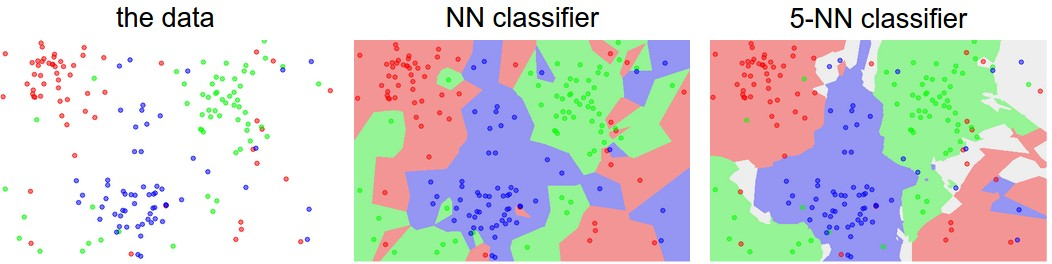
\includegraphics[scale=0.45]{kNNclf.jpg}
	\caption{The difference between NN and k-NN classiffier.}
\end{figure}

\section{Simple training algorithms}

\subsection{Perceptron}
One of the simplest "neural network" is called a Percepton. \url{https://en.wikipedia.org/wiki/Perceptron}  (.... chtělo by dodělat, pokud někdo chce ....).

\subsection{SVM - Support Vector Machine}
The idea behind SVM is to solve some problems occuring in the simple classifiers. SVM creates 2 parralel separating lines (the decision borders) which would be the furthest possible from each other. The resulting classifier then uses the middle line between these 2 created lines. It is an "optimal" linear classifier, which focuses on maximizing the margin.\\
But SVM has one fatal problem. All the line prediction depends only on some of the border items. Many times the class border data are kind of a noise and these data are usually outliers. A possible solution to this problem is to allow some mistakes (training data which will be classified wrong). A version which uses this is called the \textbf{Soft Margin SVM}. This method requires a manual setting of the allowing coefficient.

\begin{remark}
	Any classifier \textbf{should not} depend od extremal values in practice!
\end{remark}

SVM only works on linear separable data. A way how to solve non-separable data is to enlarge the dimensionality (increasing the number of features) and make them separable. There is however a \textbf{Curse of dimensionality} which says that the data soon become very sparse and a good classifier would require a lot of training data. Another option is to map the features into another space ("\textbf{The Kernel trick}"), but this might lead to over/undertraining of the model.
\begin{figure}[h]
	\centering
	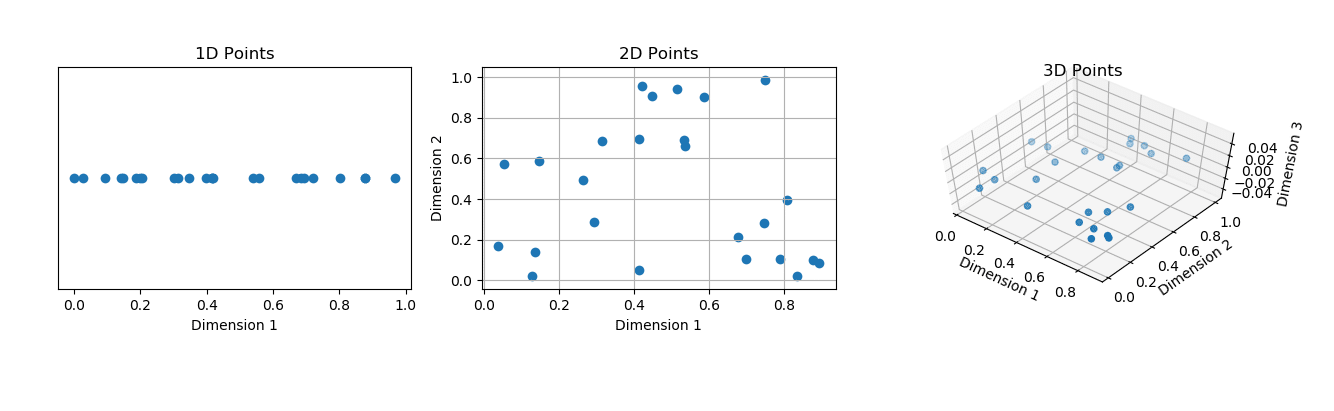
\includegraphics[scale=0.55]{Curse.png}
	\caption{Curse of Dimensionality.}
\end{figure}
\begin{figure}[h]
	\centering
	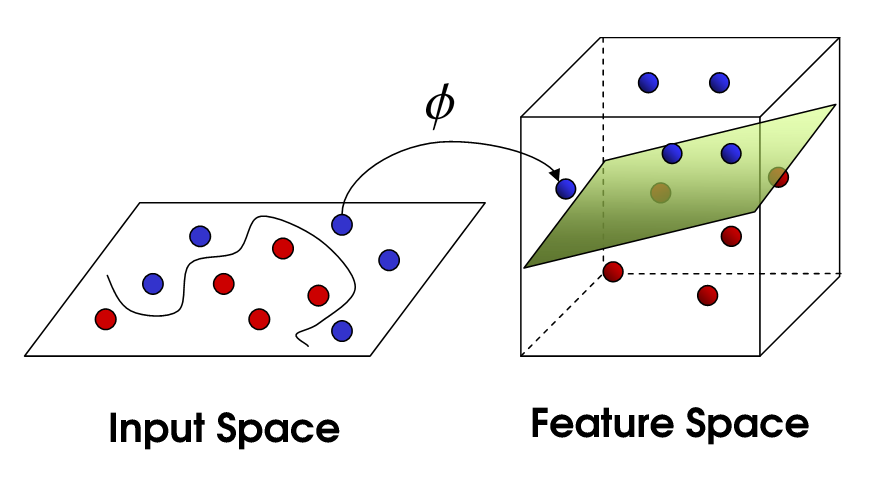
\includegraphics[scale=0.3]{KernelTrick.png}
	\caption{The Kernel trick.}
\end{figure}
\vspace{2cm}

\subsection{Classifier performance}
How to evaluate the performance of the classifiers? There are two possibilities:
\begin{itemize}
	\item evaluation on the \underline{training set} (\textbf{optimistic error estimate}) - not recommended
	\item evaluation on the \underline{test set} (\textbf{pessimistic error estimate})
\end{itemize}
In order to evaluate the performance of the classifier is to evaluate it on test set. Test dataset contains data on which the classifier did not train itself and which were chosen in the same way as the training dataset. After this we can for example calculate the \textbf{confusion matrix} or other statistics, such as accuracy, precision, recall etc. 

\begin{figure}[h]
	\centering
	\includegraphics[scale=0.35]{ConfusionMatrix.png}
	\caption{Example of a Confusion matrix.}
\end{figure}
\clearpage
\begin{remark}
	Perfect classifier would have diagonal confusion matrix. Be careful while interpreting the results given by confusion matrix - the classification classes might not be uniformly distributed and absolute numbers might be misleading. Also, in many cases (typically in medical environment), not all mistakes are considered equal and we might focus on reducing the most several ones. For example while diagnosing patient with an illness, it is desirable to have "false negative" error as low as possible, while "false positive" is usually not such a bother.
\end{remark}

One way how to choose the training and test dataset is to use the cross-validation where we choose the training and test datasets randomly and calculate particular confusion matrices. The final step is to train the classfier on all the data (and believe that it will be slightly better than all those cross-validated sets). In case that the confusion matrices are very different, something is wrong with the classifier or the data.

\chapter{Unsupervised Classification (cluster analysis)}
Clusters are hardly defined as a compact well-separated subsets of data. There is no good formal definition. One of them is e.g. that a cluster is a subset in which it is possible to jump to another item with a step smaller than some $t$. However, even a small change of $t$ can significantly affect the subsets. For this reason, no definition is used and in practise any partition of the data is considered as a cluster. Instead, algorithms are compared by how good clusters are they making.

\begin{define}[Ward criterion]
In order to compare clustering, we define Ward criterion for $N$ Clusters as
$$ J=\sum_{i=1}^N \sum_{\textbf{x}\in C_i}\left\|\textbf{x}-\textbf{m}_i\right\|^2, $$
where $\textbf{m}_i$ is a center of mass from the $i$-th cluster and $C_i$ is a set of items belonging to the $i$-th cluster.
\end{define}

In real problems the variance measure $J$ from the Ward criterion should be minimized (but not with $N$ since $\min_N J(N)$ is monotone descreasing). There are some problems with this criterion, such as when there is a small cluster and a big one, it tries to make two similar size clusters.

When $N$ is known, we can use the \textbf{Iterative methods}. When the $N$ is unknown, we can use the \textbf{Hierarchical methods}. There are also algorithms combining these two groups.

\subsection{Iterative methods}
\subsection*{N-means clustering}
In N-means clustering we choose $N$ initial cluster centroids, then we classify every point $x$ according to the minimal distance. From this we get $N$ clusters. In each of them the center of mass is computed and taken to the next iteration. The iteration ends when the centers do not move. In other words, the algorithm is following

\begin{enumerate}
	\item select N initial cluster centeroids;
	\item classify every point $\textbf{x}$ according to minimum distance;
	\item recalculate the cluster centeroids;
	\item if centeroids did not change, then STOP, else GO TO 2.
\end{enumerate}

There are many drawbacks such as the results highly depend on the initial center choice and $J$ is not minimized. Also, the results are often intuitively wrong. For this reason, it is generally a good idea to run all the process many times with different initializations. On the other hand, compared to other methods this algorithm is very fast and simple.

\subsection{Hierarchical clustering methods}
In Hierarchical clustering, we distinguish between two approaches. In the first one, \textbf{Agglomerative clustering}, we begin with as many clusters as there are items. In each step two most similar (closest) clusters are joined together. One option is to calculate the Ward criterion for every possible change and choose the one that increases the Ward criterion with a minimal possible value. On the other hand, we can use center of masses of the maximum or minimum from the items already present in the cluster. The iteration ends when a strongly defined stopping rule is met or when there is too big increase of the Ward criterion compared to the previous ones. The result can be show in a clustering tree called the \textbf{dendrogram}. Algorithm summary:
\begin{enumerate}
	\item each point = one cluster;
	\item find two "nearest" or "most similar" clusters and merge them together;
	\item repeat 2. until the stop rule is reached. 
\end{enumerate}

The second approach is called \textbf{Divisive clustering}. The difference is, that we begin with one cluster and in each step we split the cluster(s) into two smaller ones.\\

\begin{figure}[h]
	\centering
	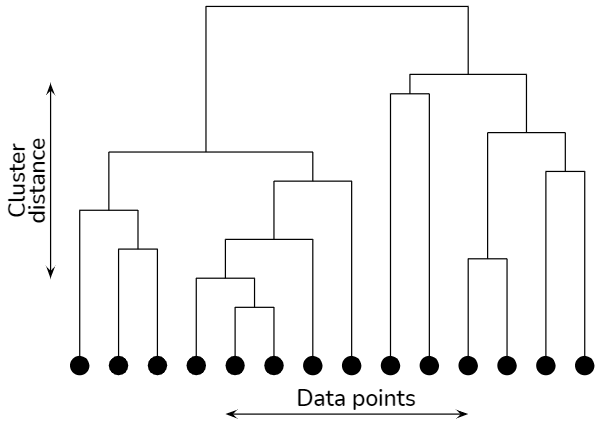
\includegraphics[scale=0.5]{dendrogram.png}
	\caption{Example of dendrogram. As a measure for cluster distance Ward statistics $J$ can be used.}
\end{figure}
